\documentclass[11pt,a4paper]{article}
\usepackage[margin=2.2cm]{geometry}
\usepackage{graphicx,booktabs,amsmath,hyperref}
\setlength{\parindent}{0pt}\setlength{\parskip}{0.6em}
\title{Auctions and the VCG Mechanism: Simulation Report}
\date{}
\begin{document}
\maketitle

All code is in \texttt{part1\_second\_price.py}, \texttt{part2\_first\_price.py} and \texttt{part3\_vcg.py}
(run with \texttt{./run\_all.sh}); raw outputs are in \texttt{results/} and figures in \texttt{figures/}.
Seeds are fixed. Every Monte-Carlo curve is overlaid with the exact expected utility, and the code
asserts that the two agree (max.\ error below 0.005; observed below 0.0015).

\section{Part 1: Second-price sealed-bid auction}

\textbf{Setup.} Bidder 1 has value $v\in\{0.2,0.5,0.8\}$ and bids $b$; it wins if $b$ exceeds the highest
rival bid $M$ and then pays $M$, so $u=(v-M)\mathbf 1[b>M]$. Each rival value is $U[0,1]$ and the rival
strategy is truthful ($M\sim U[0,1]$), half ($U[0,\tfrac12]$) or random ($U[0,1]$, independent of its value).
For each of the 9 (value, strategy) combinations I simulate $2\times10^5$ auctions for each bid
$b=0.00,0.01,\dots,1.00$. The same random rival bids are reused for every $b$ (common random numbers), which
removes sampling noise from comparisons between bids.

\subsection*{A. Utility versus bid (one rival)}
\begin{center}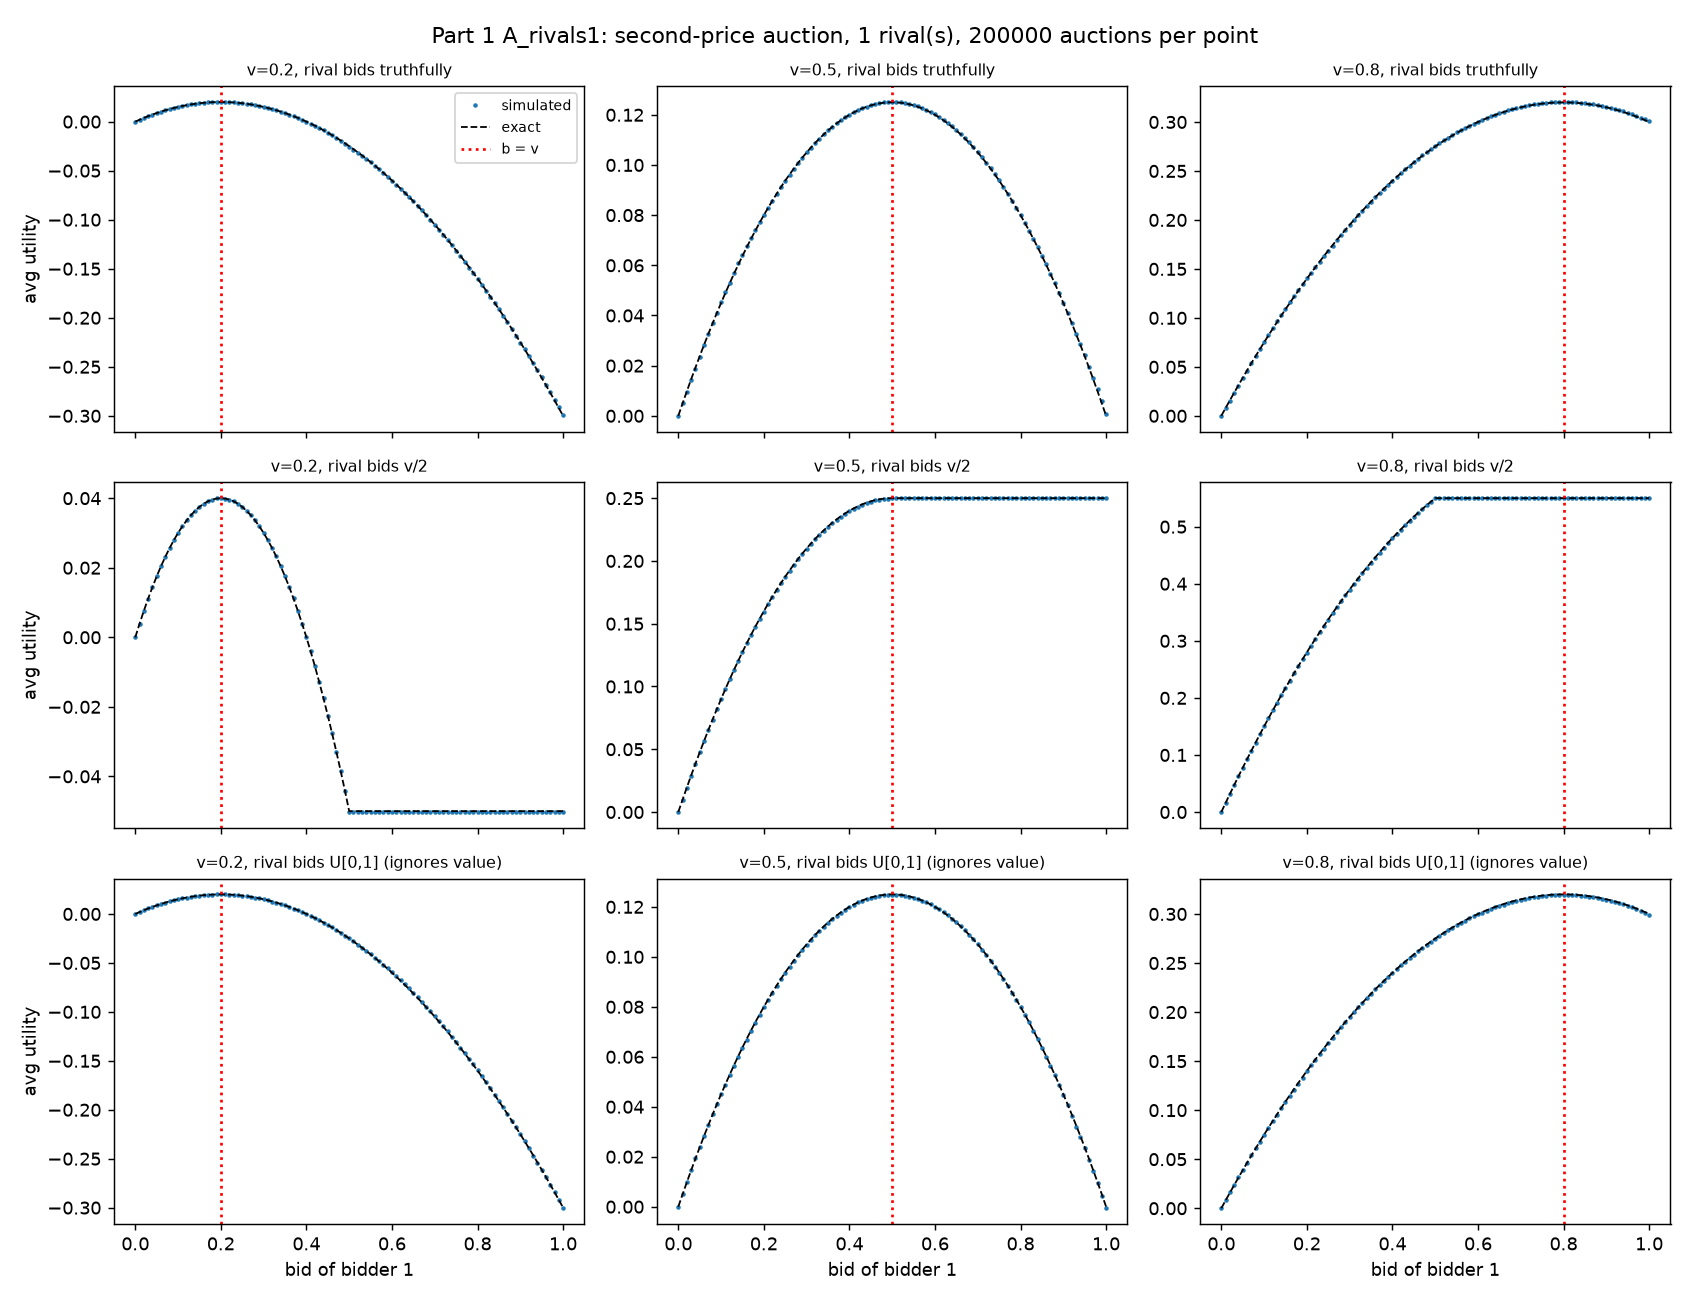
\includegraphics[width=\textwidth]{figures/part1_A_rivals1.png}\end{center}

\begin{tabular}{llrrr}\toprule
rival strategy & $v$ & best bid & max avg.\ utility & utility at $b=v$\\\midrule
truthful & 0.2 / 0.5 / 0.8 & 0.20 / 0.50 / 0.80 & 0.0201 / 0.1251 / 0.3205 & same\\
half & 0.2 / 0.5 / 0.8 & 0.20 / 0.50 / $\ge$0.50 & 0.0400 / 0.2497 / 0.5497 & same\\
random & 0.2 / 0.5 / 0.8 & 0.20 / 0.50 / 0.80 & 0.0200 / 0.1249 / 0.3195 & same\\\bottomrule
\end{tabular}

\textbf{Observations.}
\begin{itemize}
\item In all nine plots the maximum is at $b=v$ (the red line). Bidding lower than $v$ gives up auctions that are
profitable (the rival bid is below $v$). Bidding higher than $v$ wins auctions in which the price is above $v$
and so produces a loss; for $v=0.2$ against the half-bidder, bidding $\ge 0.5$ wins every auction at an
average price of $0.25$, giving utility $-0.05$.
\item The truthful and random rivals give the same curves. Bidder 1 only observes the \emph{distribution} of the
rival's bid, and in both cases it is $U[0,1]$. Whether the rival ``means'' its bid does not matter.
\item Against the half-bidder the rival bid lies in $[0,0.5]$, so for $v\ge0.5$ the curve is flat for $b\ge 0.5$:
any bid in $[0.5,1]$ wins every auction at the same price, and $b=v$ lies on this plateau (so it is a best
response, though not the unique one).
\item The exact curve is $E[u](b)=(v-b)F(b)+\int_0^b F(x)\,dx$ where $F$ is the CDF of $M$.
It is maximised at $b=v$ since $dE[u]/db=(v-b)F'(b)$ changes sign at $v$.
\end{itemize}

\textbf{Do the plots help bidder 1 choose its strategy?} They show the payoff of each bid against a given rival
behaviour, and they confirm that the best bid is $v$ in every case, but they do not help it \emph{choose}: the
best response is the same ($b=v$, or a set that contains it) against all three rival strategies, so bidder 1 does
not need to know or learn the rival's strategy. The strategy only changes how much bidder 1 earns
(e.g.\ 0.55 vs 0.32 at $v=0.8$), not what it should bid. This is the practical meaning of truthful bidding being
a weakly dominant strategy.

\subsection*{B. Fixed rival bids $\{0.1,0.4,0.9\}$}
With the rival bid $r$ fixed, $u(b)=v-r$ if $b>r$, $(v-r)/2$ at a tie (coin-flip tie-break), $0$ if $b<r$.
\begin{center}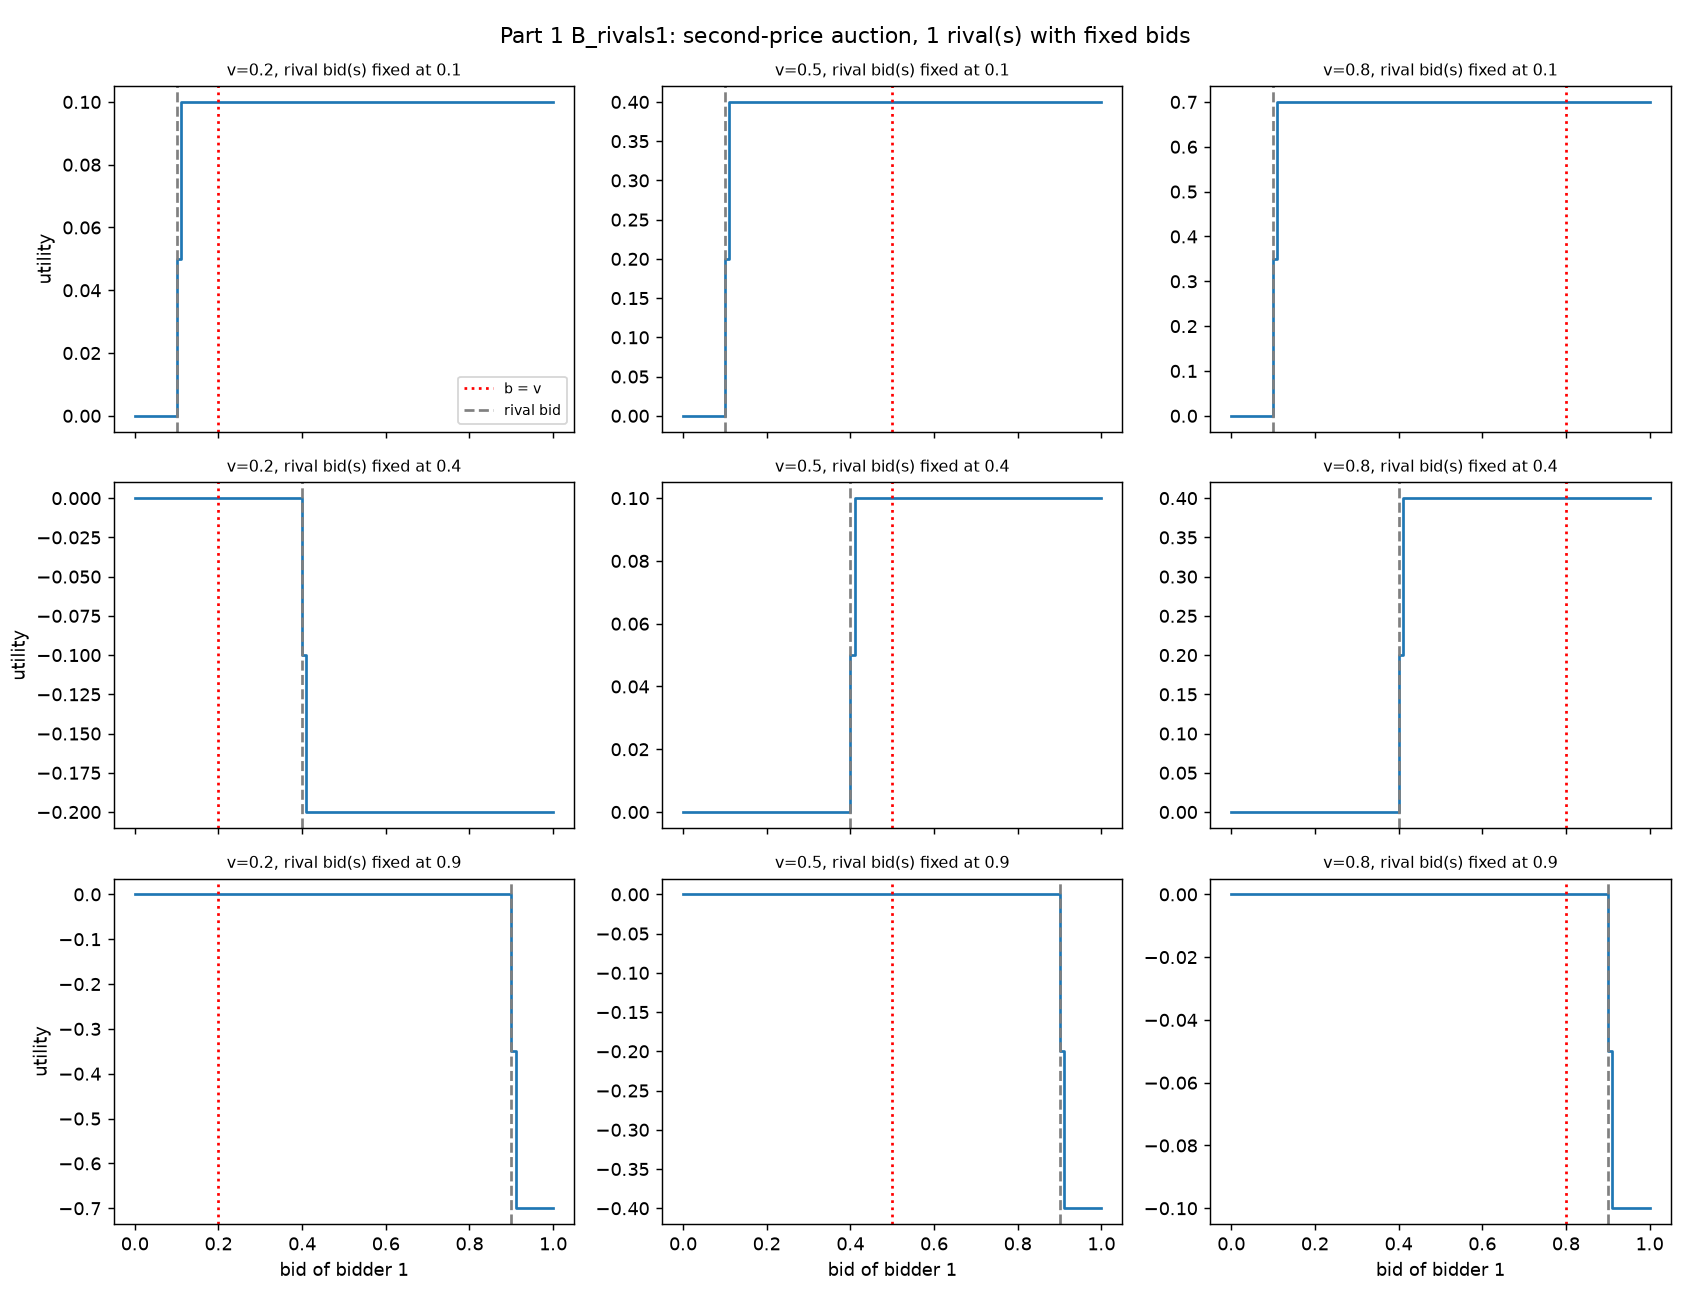
\includegraphics[width=0.85\textwidth]{figures/part1_B_rivals1.png}\end{center}
\begin{tabular}{lccc}\toprule
 & $r=0.1$ & $r=0.4$ & $r=0.9$\\\midrule
$v=0.2$ & 0.1 (win) & 0 (lose) & 0 (lose)\\
$v=0.5$ & 0.4 (win) & 0.1 (win) & 0 (lose)\\
$v=0.8$ & 0.7 (win) & 0.4 (win) & 0 (lose)\\\bottomrule
\end{tabular}

Utility of $b=v$ (entries) equals the maximum over all 101 bids in all 9 cases (checked in code).
Reason: if $v>r$, truthful bidding wins and earns $v-r$, the largest available; if $v<r$, truthful bidding loses
and earns $0$, while winning would cost $r-v>0$. Nothing the bidder does changes the price it pays, only whether it wins,
and $b=v$ wins exactly when winning is profitable.

\subsection*{C. Two rivals (bidders 2 and 3)}
The task text says ``repeat parts A and C''; I took this to mean A and B. Both rivals use the same strategy
with independent values, and bidder 1 pays $M=\max(b_2,b_3)$.
\begin{center}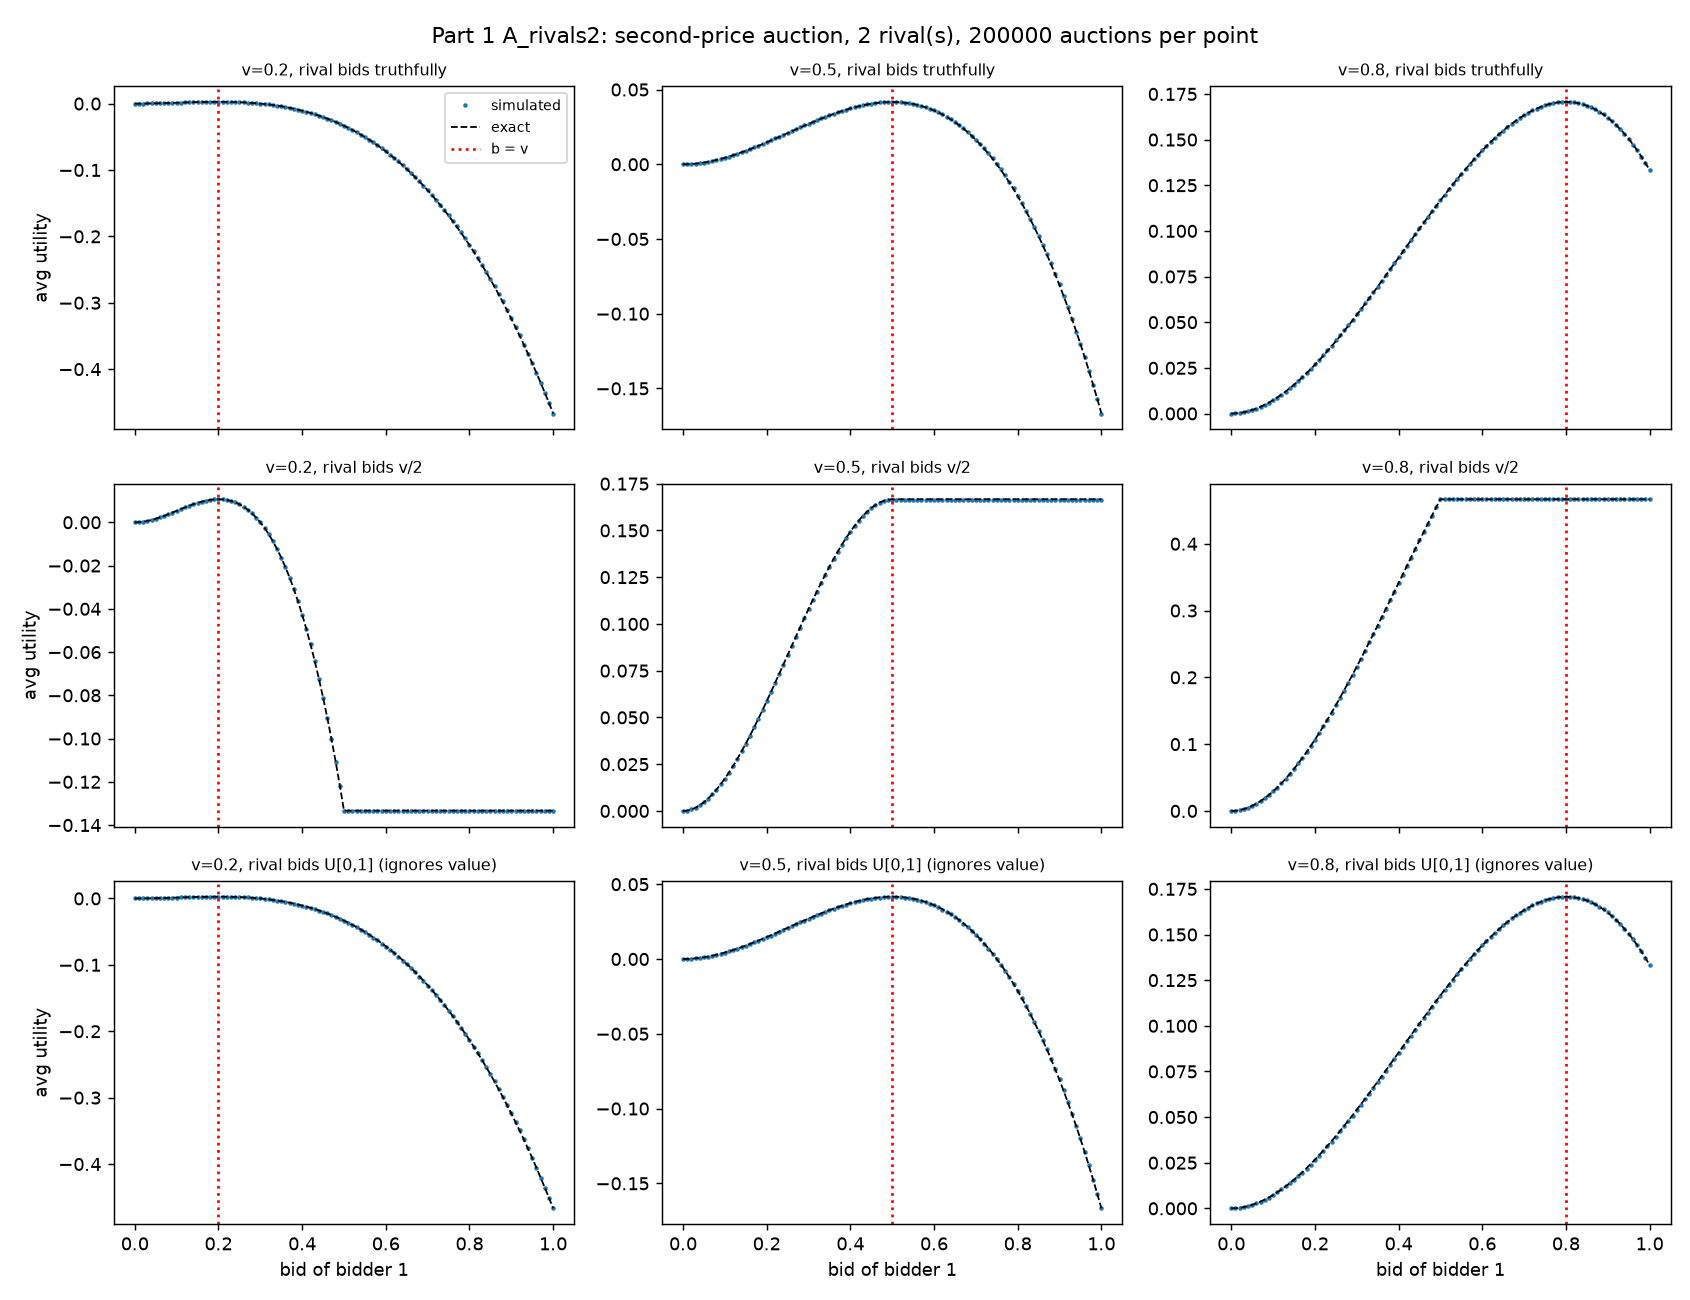
\includegraphics[width=\textwidth]{figures/part1_A_rivals2.png}\end{center}
\begin{center}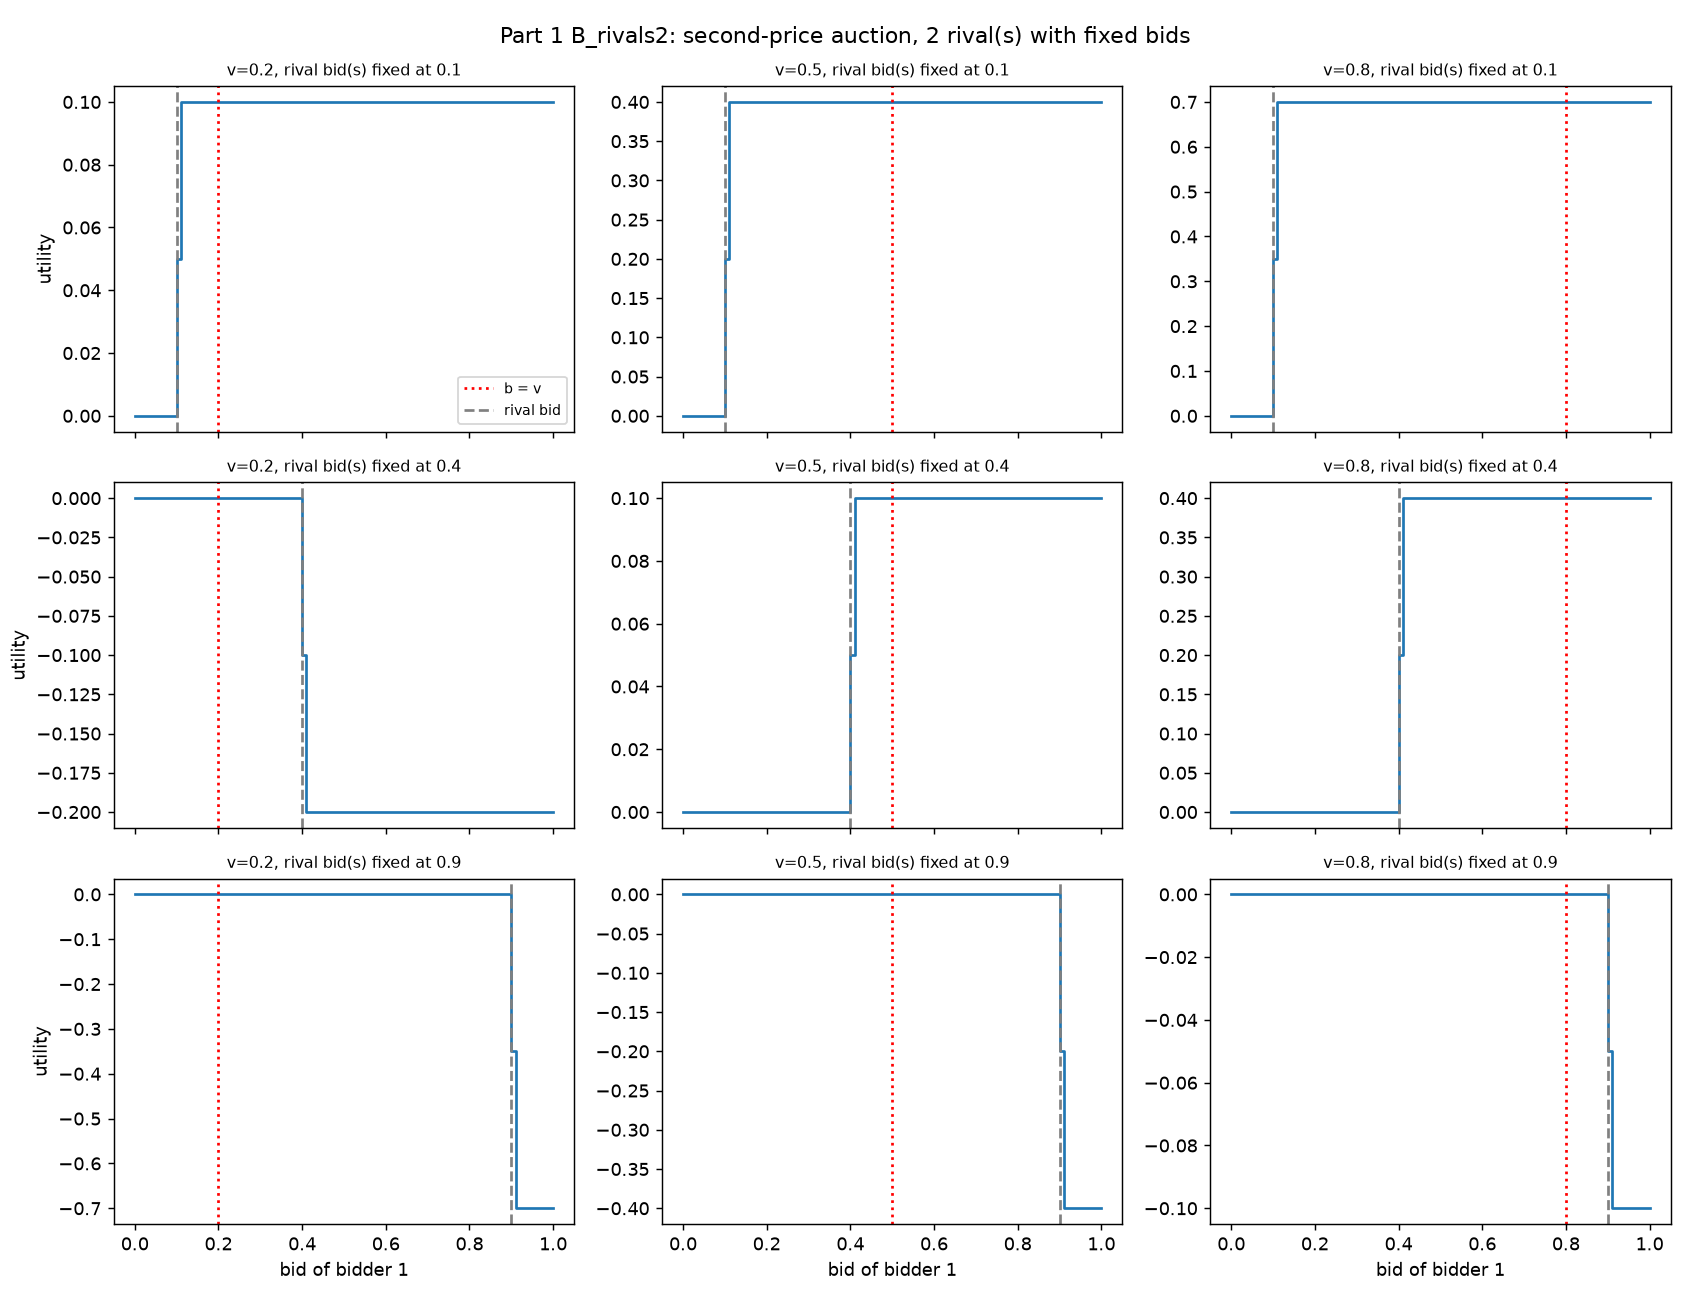
\includegraphics[width=0.85\textwidth]{figures/part1_B_rivals2.png}\end{center}
Results (all in \texttt{results/part1.txt}):
\begin{itemize}
\item The best bid is again $b=v$ in all nine cases (plateau for $v=0.8$ against the half-bidders).
Max.\ utilities: truthful 0.0027 / 0.0418 / 0.1707; half 0.0106 / 0.1665 / 0.4665; random 0.0026 / 0.0415 / 0.1707
(for $v=0.2/0.5/0.8$).
\item Utilities are much lower than with one rival (e.g.\ $v=0.8$, truthful rival: 0.3205 $\to$ 0.1707) because $E[\max]$ is higher
(2/3 instead of 1/2), so a win costs more and happens less often when $b<v$. The maximiser does not move.
\item For fixed rival bids the utility depends only on the \emph{highest} rival bid, so I checked all six pairs from
$\{0.1,0.4,0.9\}$; $b=v$ is optimal in each (the figure shows the pairs with equal bids).
\end{itemize}
Conclusion for Part 1: truthful bidding is a (weakly) dominant strategy independent of the number of rivals and of their strategy.

\section{Part 2: First-price auction with $n$ bidders}
Bidder 1 has $v\sim U[0,1]$ and bids $kv$ for $k\in\{0.1,0.2,\dots,2.0\}$; the other $n-1$ bidders bid the
equilibrium bid $\tfrac{n-1}{n}v_i$. The highest bid wins and pays its own bid. I use $2\times10^5$ auctions per
$n$. Exact expected utility: $E[u]=\int_0^1(1-k)v\,\min\!\big(1,\tfrac{knv}{n-1}\big)^{n-1}dv$, maximised at $k^*=\tfrac{n-1}{n}$ with value $\tfrac1{n(n+1)}$.
The overpayment measure for an auction is (winning bid) $-$ (second-highest bid); the winner ``could have
paid less and still won'' exactly when this is positive.

\begin{center}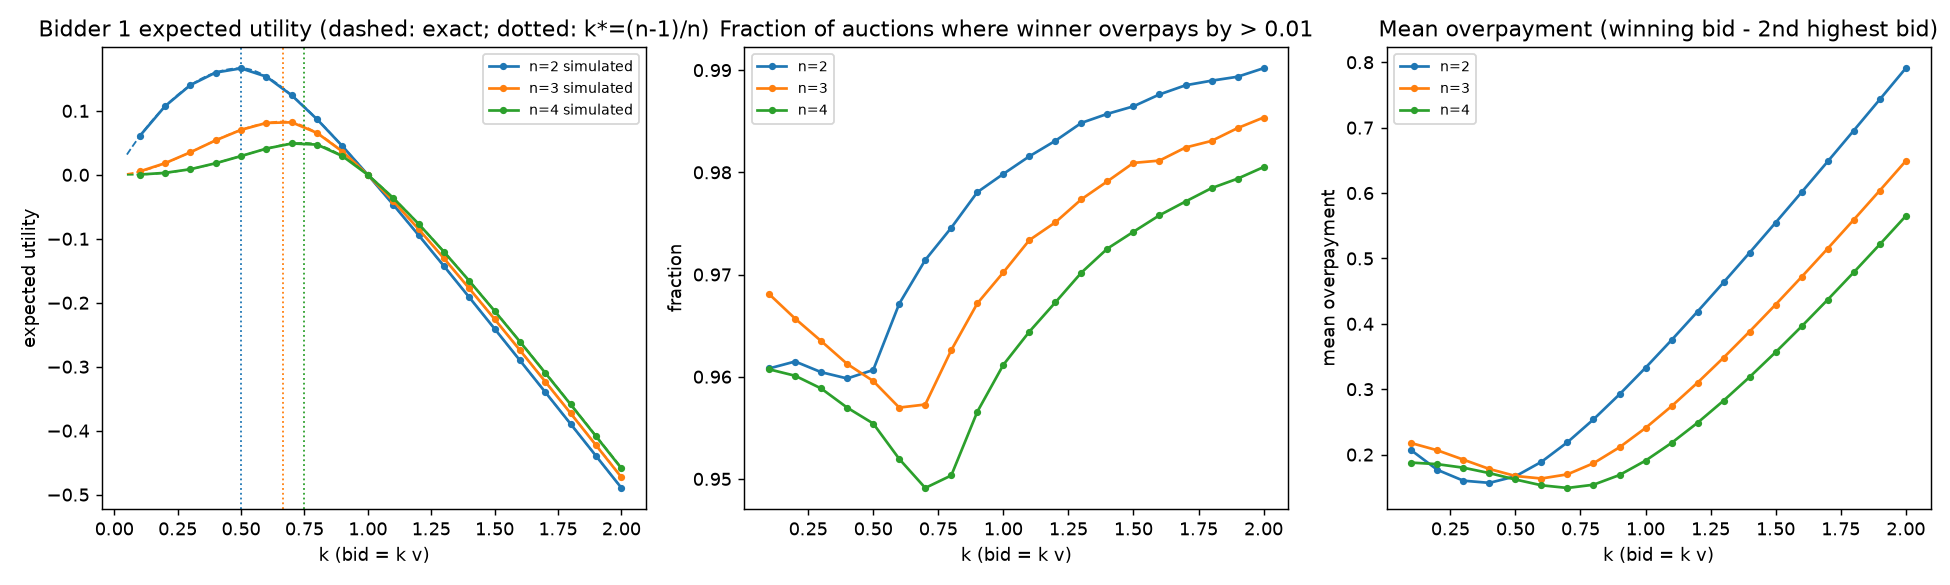
\includegraphics[width=\textwidth]{figures/part2_first_price.png}\end{center}

\begin{tabular}{crrrrrr}\toprule
$n$ & $k^*$ & best grid $k$ (sim.) & $E[u]$ at best grid $k$ & $E[u]$ at $k^*$ (exact) & $E[u]$ at $k=1$ & $E[u]$ at $k=2$\\\midrule
2 & 0.500 & 0.5 & 0.1665 & 0.1667 & 0.000 & $-0.489$\\
3 & 0.667 & 0.7 & 0.0821 & 0.0833 & 0.000 & $-0.473$\\
4 & 0.750 & 0.7 & 0.0490 & 0.0500 & 0.000 & $-0.459$\\\bottomrule
\end{tabular}

\vspace{0.5em}
\begin{tabular}{crrrr}\toprule
$n$ & & fraction overpaying ($>0$) & fraction overpaying $>0.01$ & mean overpayment\\\midrule
2 & $k=0.5$ & 1.0000 & 0.961 & 0.167\\
3 & $k=0.7$ & 1.0000 & 0.957 & 0.170\\
4 & $k=0.7$ & 1.0000 & 0.949 & 0.149\\\bottomrule
\end{tabular}

\textbf{Analysis.}
\begin{itemize}
\item \emph{Deviation does not pay.} The utility curve peaks at $k^*=(n-1)/n$ (on the grid: $k=0.5$ for $n=2$, and the nearest grid points $0.7$ for $n=3,4$, since $2/3$
and $3/4$ are not on the grid; exact value at $k^*$ is slightly higher). Shading below $k^*$ loses too many auctions; bidding above
it wins more often but at a smaller margin. At $k=1$ the utility is exactly 0 (win more often, but pay your whole value) and for $k>1$ it is negative.
\item \emph{Equilibrium shading shrinks with $n$.} More competitors make bidding close to one's value necessary ($k^*$ rises)
and cut expected profit ($1/6,1/12,1/20$).
\item \emph{Winner could have paid less: almost always.} With continuous bids a tie for the top is a
probability-zero event, so the winner's bid exceeds the runner-up's in 100\% of auctions for every $n$ and $k$; this is a feature of the
first-price rule (the winner pays its own bid rather than the second-highest). Because that fraction is degenerate,
I also report the fraction in which the saving exceeds 0.01: about 95--99\% in every case (higher for large $k$, where bidder 1 bids too high
and wins). The \emph{size} of the overpayment is more informative: about 0.15--0.17 around equilibrium (on the order of a third to a half of the winning bid);
it grows rapidly with over-bidding ($k=2$: 0.79 for $n=2$), and at equal $k$ it falls as $n$ increases because the runner-up bid
gets closer to the top bid.
\item The mean overpayment is not minimised at $k^*$ (e.g.\ for $n=2$ it is 0.160 at $k=0.3$ and 0.167 at $k^*$): it measures how much
the winner pays above the runner-up bid, not bidder 1's own utility. A second-price rule (Part 1) would charge exactly the runner-up bid, so
this overpayment is what the first-price winner must trade against the risk of losing when shading.
\end{itemize}

\section{Part 3: VCG mechanism for the cheapest path A$\to$F}
\textbf{Mechanism.} Each directed edge is an agent with a private cost $c_e$. The mechanism picks the cheapest path under reported costs and pays an
on-path agent $p_e=d(G\setminus e)-\big(d(G)-c_e\big)$ ($d$ = cost of the cheapest path, computed with the other agents' reports);
off-path agents get 0. An agent's utility is $p_e-c_e^{\text{true}}$ if selected, else 0.

\textbf{Graph.} Figure 7.3 of the book has directed edges AB=3, AC=2, BD=2, BE=1, CE=3, CF=5, DF=2, EF=1.
The paths from A to F cost ABEF 5, ACEF 6, ABDF 7 and ACF 7, so the cheapest is ABEF. The cheapest path without AB, without BE and without EF costs
6, 6 and 7 respectively.

\textbf{Reproduction.} Chosen path ABEF (cost 5). With $p_e=d(G\setminus e)-(d(G)-c_e)$: $p_{AB}=6-(5-3)=4$, $p_{BE}=6-(5-1)=2$,
$p_{EF}=7-(5-1)=3$, and 0 for all other edges, exactly as in the text (checked by assertion). Utilities when truthful: AB 1, BE 1, EF 2, others 0.

\begin{center}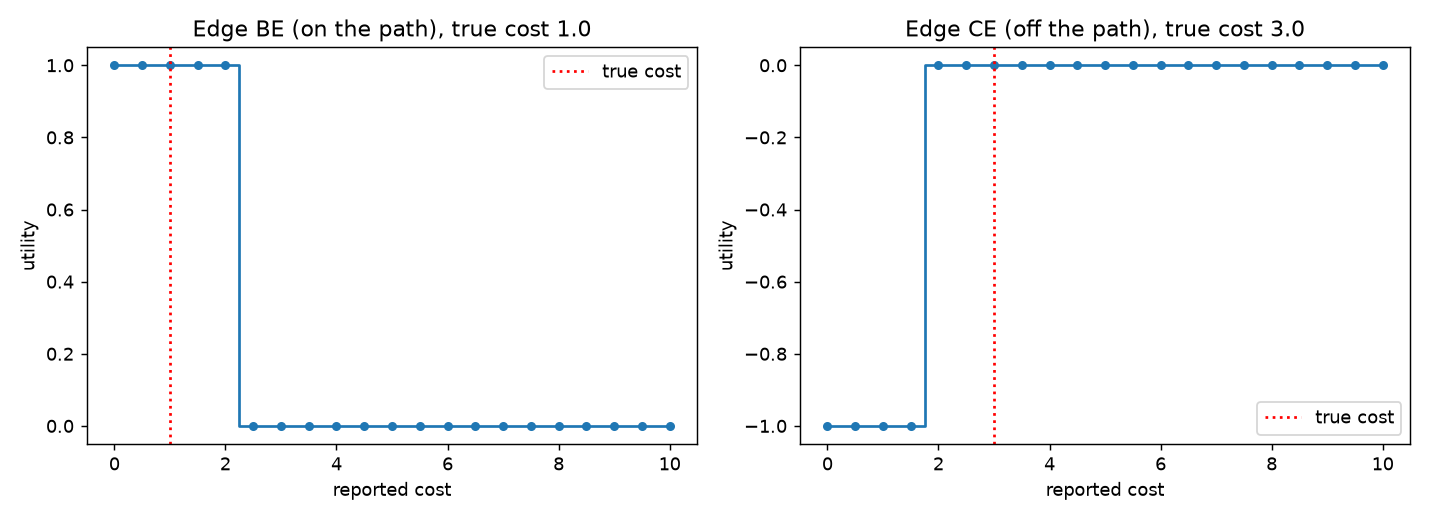
\includegraphics[width=0.9\textwidth]{figures/part3_vcg.png}\end{center}

\textbf{Edge BE (on the path, true cost 1).} Reports 0 to 2 give utility 1, reports of 2.5 and above give 0.
The payment to a selected agent (2) does not depend on its own report; the report only determines whether it is selected,
and it stays selected as long as the path through it is no more expensive than the next best path (reports up to 2). Lying low
changes nothing, lying high loses a profitable sale.

\textbf{Edge CE (off the path, true cost 3).} Reports 0 to 1.5 make CE part of the cheapest path (ACEF), but the
payment is then only 2, below its true cost 3, so its utility is $-1$. Reports $\ge2$ leave it off the path, utility 0. Truthful
reporting gives utility 0, the best among the options. (At the tie report 2 the code breaks ties by the lexicographically first path, ABEF.)

I also checked every one of the 8 edges against all 21 reports $0,0.5,\dots,10$: the truthful report always maximises utility,
so VCG is dominant-strategy truthful here, and agents on the path earn a strictly positive rent (1, 1, 2), which is the price of truthfulness.
The total payment of 9 exceeds the true cost 5 (``overpayment'' of the VCG mechanism).

\section{Interactive simulation}
The folder \texttt{simulation/} contains a browser app (open \texttt{simulation/index.html}; it runs offline) that re-implements the same
experiments with the same exact formulas (\texttt{core.js}, mirroring the Python scripts) and lets one explore them:
\begin{itemize}
\item \emph{Second-price tab:} a live auction replay (bid bars, winner, price, running profit), the utility-versus-bid curve with simulated points
accumulating over the exact curve, a convergence plot of the estimate $\pm1.96$ standard errors against the number of auctions,
a ``fixed rival bid'' mode for Part B with an automatic check that $b=v$ is optimal over all 101 bids, a regret heatmap over (value, bid), and the $3\times3$ grid of Part A.
\item \emph{First-price tab:} live replay with the overpayment of each winner, expected utility versus $k$ for $n=2,3,4$, mean overpayment and the
histogram of overpayments at the chosen $k$.
\item \emph{VCG tab:} the graph of Figure 7.3 with editable edge costs, the chosen path animated, payments and utilities updated live, and the misreport experiment
for any selected edge.
\end{itemize}
The browser results agree with the Python results: for $v=0.8$ against a truthful rival 100{,}000 auctions give 0.3194 (exact 0.3200); for $n=2$, $k=0.5$ they give
0.1669 (exact 0.1667) and 96.1\% of winners could have paid more than 0.01 less; the VCG tab reproduces ABEF with payments 4, 2, 3.

\end{document}
